\section{Aufbau und Durchführung}
Der Versuchsaufbau ist in Abbildung~\ref{fig:aufbau} dargestellt. Die verwendete Lichtquelle ist eine Halogen-Lampe, da ihr Emissionsspektrum
zu großen Teilen im Infrarotbereicht liegt. Dies wird benötigt um nur Verschiebungspolarisationen zu betrachten. Zunächst wird der Lichtstrahl durch
eine Linse gebündelt und anschließend durch einen Lichtzerhacker in Impulse unterteilt. Dies hat den Vorteil, dass das Rauschen, dass durch den hohen
Innenwiderstand der zur Messung verwendeten Photowiderstände entsteht, zu vermindern. Dafür wird der Selektivverstärker auf die Frequenz des Zerhackers eingestellt.
Anschließend wird der Lichtstrahl durch ein drehbares Glan-Thomson-Prisma geleitet, wodurch nur noch zwei linear polarisierte, zueinander senkrechte Lichtstrahlen
erhalten werden. Davon wird jedoch nur einer in einen Elektromagneten geleitet, in dessen Mitte sich die Probe befindet. Nachdem der Strahl aus
diesem wieder austritt, durchläuft er einen Interferenzfilter und wird dann erneut durch ein Glan-Thomson-Prisma aufgeteilt. Die beiden Strahlen treffen
anschließend auf zwei Photowiderstände. Die beiden Signale werden an einen Differenzverstärker weitergeleitet, der anschließend das Signal an den Selektivverstärker
angeschlossen ist. Das Signal wird dann schließlich mit Hilfe eines Oszilloskopes dargestellt.\\

\begin{figure}
  \centering
  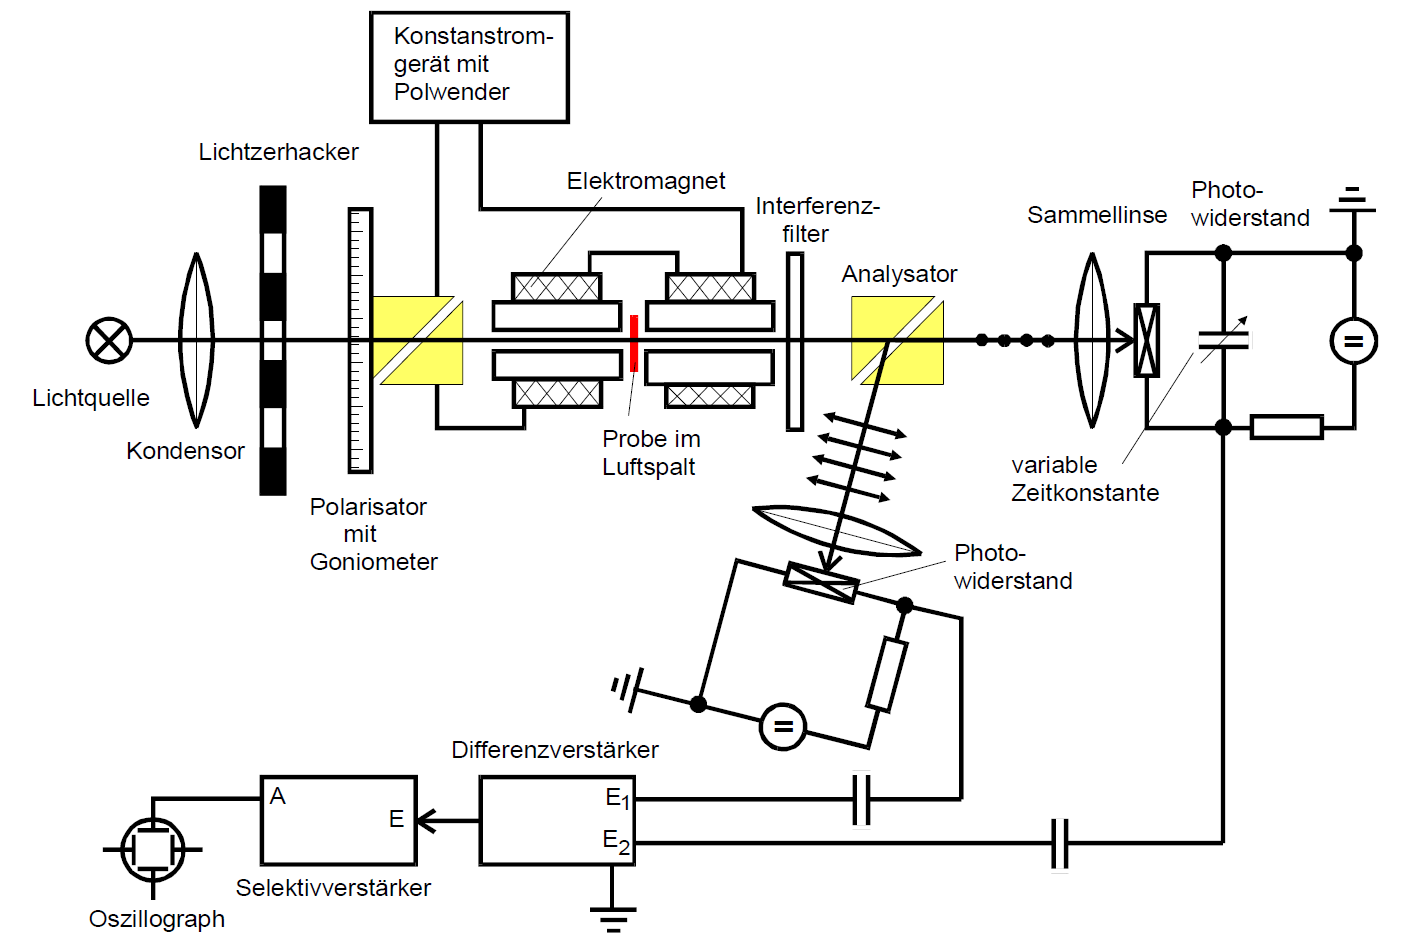
\includegraphics[scale=0.35]{graphics/aufbau.png}
  \caption{Schematische Darstellung des Versuchsaufsbaus.}
  \label{fig:aufbau}
\end{figure}

Zu Beginn des Versuchs muss dieser erst justiert werden. Dabei ist darauf zuachten, dass die Photowiderstände so ausgerichtet sind,
dass bei einem leeren Strahlengang die Intensitätsmaxima genau auf diese beiden treffen. Zudem sollten die Frequenz des Zerhackers und des
Selektivverstärkers übereinstimmen.
Anschließend wird die Lampe auf etwa $\SI{12}{\volt}$ eingestellt und eine Leermessung gemacht, bei dieser wird das Goniometer so eingestellt,
dass sich die beiden Intensitäten bestenfalls auslöschen. Dieser Winkel wird notiert. Nun wird der Elektromagnet langsam hoch gefahren, um
Induktionsströme zu findern.
Mit diesem Aufbau werden nun drei Proben, eine undotierte Galliumarsenid (GaAs) und zwei verschiedene n-dotierte GaAs-Proben, mit jeweils
acht verschiedenen Interferenzfiltern vermessen. Dafür wird mit dem oben beschriebenen Vorgehen der Winkel bestimmt und notiert. Anschließend
wird das Magnetfeld noch einmal umgepolt und das gesamte Vorgehen wiederholt. Aus der Differenz lässt sich anschließend der Faradaywinkel
$\vartheta = \vartheta_1 - \vartheta_2$ bestimmen.
Zum Schluss wird die Probe entfernt und mit einer Hallsonde das Magnetfeld vermessen, um die magnetische Feldstärke im Bereich der Probe zu bestimmen.
